\chapter{When the method is exact}
\label{ch:exactness}

% Added 2026-09-24.  Every number is read off statmech/probe/results/
% acyclicity_{rgg,hrg,fss}.csv and real_acyclicity.csv; see book/extensions.md
% for the plan this chapter carries out.

Part~IV so far has measured where the recursion fails, repaired it one
instance at a time, and identified the cause as complexes sharing two or more
atoms. This chapter turns that around. The condition under which the
calculation is exact has a name, in fact three, and once it is named the
question stops being ``how large is the error'' and becomes ``on which
ensembles is there none''. The answer is a transition of the same kind as the
core percolation of Chapter~\ref{ch:cover}, with leaf removal once more as the
certificate, run this time on the incidence structure rather than on the
graph.

\section{Three names for one condition}
\label{sec:threenames}
\index{chordal graph|textbf}
\index{acyclic hypergraph|textbf}
\index{join tree|textbf}
\index{GYO reduction|textbf}

Take a graph $G$ and the family $\mathcal{C}$ of its maximal cliques, which is
the chygraph Chapter~\ref{ch:data} builds from it. Three statements about
$(G,\mathcal{C})$ turn out to be the same statement.

\emph{The graph is chordal.} Every cycle of length four or more has a chord,
an edge between two vertices of the cycle that is not itself an edge of the
cycle \citep{dirac1961}. Two triangles sharing an edge are chordal: the
four-cycle through their outer vertices has the shared edge as its chord. A
four-cycle on its own is not, and neither is a wheel whose rim has four or more
spokes, which is the structure Chapter~\ref{ch:overlap} found around the
vertices of a real network.

\emph{The clique family has a join tree.} There is a tree $T$ whose vertices
are the maximal cliques such that, for every atom $v$, the cliques containing
$v$ form a connected subtree of $T$ --- the running intersection property.
Gavril proved that the graphs whose maximal cliques can be arranged this way
are exactly the chordal graphs \citep{gavril1974}; in the language of
hypergraphs the clique family is then $\alpha$-acyclic, the weakest of the
acyclicity notions of \citet{beeri1983} and the one that matters for
computation.

\emph{Leaf removal on the incidence structure consumes everything.} Delete an
atom that lies in one clique only; delete a clique contained in another;
repeat. This is the GYO reduction of \citet{graham1979} and \citet{yu1979}, and
it empties the family if and only if the family is $\alpha$-acyclic
\citep{beeri1983}; \citet{tarjan1984} run it in linear time. The rule is
Chapter~\ref{ch:cover}'s leaf removal applied to the bipartite graph of atoms
and complexes, with one addition --- a complex swallowed by another is removed
--- that never fires on a graph, because no edge contains another, and fires
constantly on a clique family. What GYO leaves is the \emph{residue}: the
atoms and complexes that no join tree covers.

The three are one condition, and the condition is the one Part~IV has been
circling. Chapter~\ref{ch:gbp} found the region-graph calculation exact on
every chordal instance and on no other; Chapter~\ref{ch:metacomplex} found the
merged calculation exact whenever the merged incidence structure is a forest.
Both are corollaries of the junction-tree theorem \citep{lauritzen1988}: on a
join tree, passing messages between adjacent cliques through their
intersection --- the \emph{separator} --- computes every marginal and the
partition function exactly, at a cost of $2^{c}$ per clique and nothing more.
The chygraph recursion of Chapter~\ref{ch:statmech} is that message passing in
the case where every separator is a single atom, so that the incidence
structure is itself a tree (Berge-acyclic, in the hypergraph vocabulary), and
Chapter~\ref{ch:metacomplex}'s merging is the device that enlarges complexes
until separators are single atoms again. The separator is the object the book
has been missing: a set of atoms that is neither a complex nor an atom, and
that a two-level chygraph represents as a complex of level one inside a
complex of level two --- the freedom of Sec.~\ref{sec:flatteningcost}, used
here for the first time outside satisfiability.

\paragraph{The statement.} Let $\mathcal{C}$ be the maximal cliques of $G$.
The following are equivalent: $G$ is chordal; $\mathcal{C}$ has a join tree;
GYO reduction of $\mathcal{C}$ leaves no residue; and message passing over
$\mathcal{C}$ with messages on separators computes $\ln Z$ of every Markov
random field on $G$ exactly. The chygraph recursion with messages on atoms is
exact iff, in addition, every separator is a single atom, and
Chapter~\ref{ch:metacomplex}'s merged recursion is exact iff the merge closure
of $\mathcal{C}$ has that property.

Nothing in the statement is new; it is Dirac, Gavril, Beeri--Fagin--Maier--%
Yannakakis and Lauritzen--Spiegelhalter placed side by side. What is new is
where it puts the book. Every calculation of Parts~II and~III is a
join-tree calculation on an ensemble whose join tree is assumed; Part~IV
measures what happens when the assumption fails; and the statement says the
failure has a certificate that costs linear time to run.

\section{A residue is not an obstruction}
\label{sec:residue}

The certificate is exact on an instance and useless on an ensemble, for the
same reason the tree assumption of Chapter~\ref{ch:introduction} is false on
every random graph with a giant component and right on all of them. GYO
keeps every cycle, and above the percolation threshold every graph has cycles
--- long ones, of length growing with $\ln n$, which the cavity method does
not mind. Table~\ref{tab:realresidue} makes the point on the sixteen networks
of Chapters~\ref{ch:data} and~\ref{ch:overlap}: the residue is between
$13$ and $100$ per cent of the vertices on every one of them, and it is
one connected piece. On the power grid it is $61$ per cent, and the power
grid is the network on which the plain cavity method is closest to exact,
because its loops are long.

What the recursion needs is local. A chordless cycle is a loop between
complexes that no complex contains --- the chygraph's version of the short
loop the tree assumption forbids --- and, as on a graph, a loop of length
growing with $\ln n$ costs the recursion nothing while a loop of bounded
length costs it exactness. The ensemble-level residue is therefore
\begin{equation}
  \phi=\Pr\bigl[v\ \text{lies on a chordless cycle of length four or five}\bigr],
  \label{eq:phishort}
\end{equation}
the two shortest lengths, found from $v$ in time quadratic in its degree: a
chordless four-cycle through $v$ is a pair of non-adjacent neighbours with a
common neighbour outside $N[v]$, a chordless five-cycle a pair joined by an
edge outside $N[v]$ with no shortcut. On a locally treelike graph $\phi\to0$;
on a chygraph treelike over complexes $\phi\to0$; on an ensemble where
complexes overlap in loops $\phi$ stays finite as $n\to\infty$, and the GYO
residue, which counts the long cycles too, says nothing about which of the
two one is looking at. Table~\ref{tab:realresidue} carries both columns.

A second local quantity is worth keeping beside $\phi$ because it is what
Chapter~\ref{ch:overlap} was closest to measuring. Call $v$ the hub of a
\emph{wheel} if its neighbourhood $N(v)$, on its own, contains a chordless
cycle: four or more complexes around one atom, closing a loop. This is the
same as the ball of radius one around $v$ failing to be chordal, since a cycle
through $v$ itself always has a chord. It is not Chapter~\ref{ch:overlap}'s
criterion. Two triangles sharing the edge $vb$ --- the smallest structure
Sec.~\ref{sec:threeclasses} flags, since the complexes share two atoms ---
leave $N(v)$ a path, and the join tree handles them exactly; the wheel is what
the join tree cannot absorb, and $\phi_{\mathrm{wheel}}\le\phi$ always, since
the rim of a wheel is a short chordless cycle.

The obstruction, when there is one, comes in islands: the connected
components of the set of vertices on short chordless cycles. An island of bounded
size is a meta-complex in the sense of Chapter~\ref{ch:metacomplex}, summed
exactly at a cost exponential in its size, and a chygraph whose islands are
all bounded is exact after that summation. The transition that matters is
therefore not $\phi>0$ but the percolation of the islands: the
appearance of a giant component of locally non-chordal vertices, past which
no finite summation recovers exactness. Call it \emph{acyclicity percolation}.
It sits beside core percolation as a second transition certified by leaf
removal, on the incidence structure instead of the graph.

\section{Which ensembles are exact}
\label{sec:whichexact}
\index{acyclicity percolation|textbf}
\index{random geometric graph}
\index{interval graph}

Figure~\ref{fig:acyclicity} measures $\phi$, and the largest connected piece
of the set it counts, on the ensembles the book has used and on two it has
not, all at $n=20000$; Table~\ref{tab:realresidue} does the same on sixteen
real networks. The sweeps are \code{statmech/\allowbreak probe/\allowbreak
acyclicity.\allowbreak py} and \code{real\_\allowbreak acyclicity.\allowbreak
py}.

\paragraph{Karrer--Newman is exact at every branching ratio.} Start with the
placed ensemble of Sec.~\ref{sec:coretransition}, single edges and triangles
dropped on random atoms. Two placed triangles share an edge with probability
of order $n^{-2}$ per pair, so the number of vertices on a short chordless
cycle is a constant: $157$, $149$ and $129$ at $n=5000$, $20000$ and $80000$
with $s=t=1$, which is $\phi=0.031$, $0.0075$ and $0.0016$, falling as $1/n$.
The ensemble is treelike over complexes in the limit at every $b$, and the
core that appears at $b=1$ is the giant component of the incidence structure
--- the point past which loops exist, all of them long --- and not the
boundary of exactness. That places Sec.~\ref{sec:coretransition} correctly:
it locates where an \emph{instance} stops being a forest, which is what the
instance calculations of Chapter~\ref{ch:gbp} needed, and it is silent about
the ensemble, which is exact throughout. It also explains, after the fact, why
every failure Chapter~\ref{ch:gbp} found was on a hyperbolic or a real
instance and none on a placed one.

\paragraph{Extensive overlap needs geometry.} Take $n$ points uniformly in the
unit cube of dimension $d$ and join two at distance below $r$, with
$r$ set by $\ave{k}=nV_{d}r^{d}$ \citep{penrose2003}. Every triangle of
neighbours closes, transitivity is $3/4$ in $d=1$ and $1-3\sqrt3/(4\pi)=0.586$
in $d=2$, and the maximal cliques overlap along every edge of the space. This
is the ensemble the tree assumption was invented to exclude.

In $d=1$ the graph is an interval graph \citep{scheinerman1988}, chordal by
construction: a chordless cycle would need an interval that leaves the line
and comes back. So $\phi\equiv0$ at every density (Fig.~\ref{fig:acyclicity},
squares), every ball is a path of cliques, and the join-tree calculation is
exact on a network with transitivity $3/4$. Sec.~\ref{sec:exactness-checks}
runs it: on sixteen-vertex lines the region-graph message passing of
Chapter~\ref{ch:gbp} over the maximal cliques returns $\ln Z$ to $10^{-6}$ on
every instance, where the node-level Bethe count is off by $13$ to $22$ and
the chygraph count with atom messages by up to $8$. The atom-message recursion
is not exact here because consecutive cliques share more than one atom; the
merge closure of Chapter~\ref{ch:metacomplex} repairs that at a bounded price,
its largest meta-complex being $13$ atoms in $20000$ at $\ave{k}=6$. One
subtlety is in the checks: the line, not the ring. Closing the line into a
circle adds one chordless cycle through every clique, which GYO keeps and
which is harmless, being of length $n/\ave{k}$.

In $d=2$ the picture changes at every density. Four points at the corners of
a square of side just under $r$ form a chordless four-cycle whenever the
diagonal exceeds $r$, and a Poisson process supplies such squares at a rate
proportional to $n$, so $\phi$ is finite for every $\ave{k}>0$:
$0.081$ at $\ave{k}=3$, $0.17$ at $4$, $0.28$ at $5$, $0.42$ at $6$ and
$0.84$ at $10$ (circles). The recursion is never exact in the limit. It is
nevertheless exact at a finite cost over a whole window of densities,
because the vertices on short chordless cycles come in islands and the
islands are small: mean size $11$ at $\ave{k}=4$, $19$ at $5$ and $48$ at $6$, taken over
the vertices in them, which is the cardinality of the meta-complex to sum. What
ends the window is the percolation of the islands. Figure~\ref{fig:fss} shows
the largest island against $\ave{k}$ at three sizes: from $\ave{k}=4$ to $7$
its fraction of $n$ falls with $n$ --- $0.0044$, $0.0020$, $0.0006$ at
$\ave{k}=4$ and still $0.063$, $0.036$, $0.015$ at $\ave{k}=7$, for
$n=5000$, $20000$, $80000$ --- while at $\ave{k}=9$ it does not ($0.75$,
$0.76$, $0.75$), and $\ave{k}=8$ is the crossing, $0.54$ at the two smaller
sizes and $0.29$ at the largest. The threshold $\ave{k}_{a}$ is a little
below $8$. The graph itself
acquires a giant component at $\ave{k}=4.512$ \citep{penrose2003}. Between
the two the network has a giant component, is clustered, and is not treelike
at any level the graph can see, and the chygraph calculation with finite
meta-complexes is exact on it. Above the second threshold no finite summation
suffices. That second threshold is acyclicity percolation, and it is the
transition Sec.~\ref{sec:residue} promised: certified by leaf removal on the
incidence structure, with the same continuous onset core percolation has on
the graph.

In $d=3$ the same two thresholds sit closer together. $\phi$ is $0.048$,
$0.14$, $0.29$ and $0.62$ at $\ave{k}=2$, $3$, $4$ and $6$ (triangles), the
graph percolates at $\ave{k}=2.736$ \citep{penrose2003}, the largest island
still vanishes with $n$ at $\ave{k}=4.5$ ($0.053$, $0.044$, $0.012$) and
holds $0.60$ of the vertices at $\ave{k}=6$ at all three sizes, so
$\ave{k}_{a}$ lies between $4.5$ and $6$. Higher dimension supplies more
chordless squares per vertex --- the diagonal of a square exceeds $r$ more
often when there is more room --- and the window of finite-cost exactness
narrows, from three units of mean degree in the plane to about two in
space.

\paragraph{Hyperbolic random graphs are exact outside the centre.} The
hyperbolic ensemble of Sec.~\ref{sec:hrg} at $\tau=2.5$ (light circles) has
$\phi=0.0002$, $0.006$, $0.028$ and $0.11$ at $\ave{k}=1$, $2$, $4$ and $8$,
and at every density the set is one connected piece: the largest island
holds $0.0002$, $0.005$, $0.027$ and $0.11$ of the vertices, which is all of
$\phi$. The piece is the centre of the disc. Two vertices at radii $r_{i}$,
$r_{j}$ connect when their angular separation is below
$2e^{(R-r_{i}-r_{j})/2}$, so at the periphery the graph is one-dimensional
--- an angular window of size $e^{-r/2}$, which is why Chapter~\ref{ch:gbp}
found its chordal instances there --- and near the centre the windows are of
order one, the angular coordinate closes on itself, and chordless cycles run
around it. The fraction of vertices within a fixed distance of the centre is
set by $\alpha=(\tau-1)/2$ and does not vanish with $n$, so $\phi$ is
extensive and small, and it sits where the hubs are. The exponent of
Sec.~\ref{sec:hrg} was measured on the core, which is the one region the
calculation is not exact on; the qualification in
Sec.~\ref{sec:establishes} has found its cause.

The tail decides whether the loops gather or scatter. At $\tau=3$
(triangles) $\phi$ is $0.0009$, $0.004$, $0.031$ and $0.18$ at the same
four densities and the largest piece holds half of it at $\ave{k}=4$ and
nearly all at $8$; at $\tau=4$ (light squares) $\phi$ is about the same,
$0.0006$ to $0.16$, and the largest piece is $0.001$ and $0.013$ at
$\ave{k}=4$ and $8$, the loops sitting in islands of eight and sixty. With a
light tail there is no centre to gather them, the radii still vary enough
that the angular kernel is a product $e^{-r_{i}/2}e^{-r_{j}/2}$ rather than
the sum an interval graph would need, and the result is what $d=2$ geometry
gives below its threshold: finite islands, exact at a finite cost.

The same sweep settles a question Chapter~\ref{ch:metacomplex} left open. The
merge closure --- merge complexes sharing two atoms, to convergence ---
absorbs $0.028$, $0.16$, $0.46$ and $0.84$ of the vertices into its largest
meta-complex at $\ave{k}=1$, $2$, $4$, $8$ on the same graphs, against a
$\phi$ of $0.0002$ to $0.11$. Merging over-repairs by a factor of up to
sixteen, because a chain of cliques along the angular coordinate shares two
atoms link by link without ever closing a loop, and the closure follows the
chain to the end. Sec.~\ref{sec:mergeerror}'s ``always a forest'' was
measured on ego-networks of at most twenty vertices, where the chain is
short. On the whole graph the merged recursion is exact and unaffordable;
the join tree passes through the chain at $2^{c}$ per clique.

\paragraph{Real networks: what the rewired control says.} Table~%
\ref{tab:realresidue} gives $\phi$ on the sixteen networks of
Chapters~\ref{ch:data} and~\ref{ch:overlap}, each against the mean over five
configuration-model rewirings with the same degree sequence --- the control
Sec.~\ref{sec:threads} insists on. It separates the networks into three
classes that the transitivity column alone does not.

Where the clustering is generated by groups the real network has \emph{far
fewer} short chordless cycles than its rewiring: co-authorship $0.077$
against $0.77$, \emph{Les Mis\'erables} $0.31$ against $0.75$, Collins
$0.47$ against $0.89$, and Facebook, whose friendships behave like groups,
$0.72$ against $0.92$. Promoting the groups to complexes absorbs the loops
that the degree sequence would otherwise force, and on the co-authorship
network the $0.077$ that remain sit in islands of fifteen: this is the
chygraph's home, and it is exact there at a finite cost.

On the seven interactomes $\phi$ is within a few hundredths of its control
($0.18$ against $0.25$ for yeast, $0.49$ against $0.53$ for Vidal, $0.52$
against $0.53$ for Figeys) and it percolates. These loops are the ones the
degree sequence makes at this $n$ --- squares through hubs, the finite-size
loops every ensemble calculation on a graph already ignores --- and the
chygraph neither adds to them nor removes them. The recursion is as exact
here as it is on any sparse graph, which is to say in the limit and not on
the instance.

On the two spatial networks the sign reverses: the power grid has
$\phi=0.29$ against $0.02$ and Euroroad $0.26$ against $0.02$. These loops
are geometry, as in $d=2$, and as in $d=2$ below $\ave{k}_{a}$ they do not
percolate --- the largest piece is $0.07$ and $0.10$ of the vertices, in
islands of $187$ and $71$. Exact in principle, at a price set by the island.

Two columns of the table say nothing, and are there to say so. The GYO
residue is between $0.13$ and $1$ on every network, including the power
grid at $0.61$, because it counts the long cycles; and the wheel fraction
$\phi_{\mathrm{wheel}}$ is below $0.03$ on every sparse network, so the
structure Chapter~\ref{ch:overlap} came closest to measuring is not where
the obstruction is. The obstruction is the chordless square, which no
clustering coefficient sees and every rewiring makes.

\begin{figure}[t]
\centering
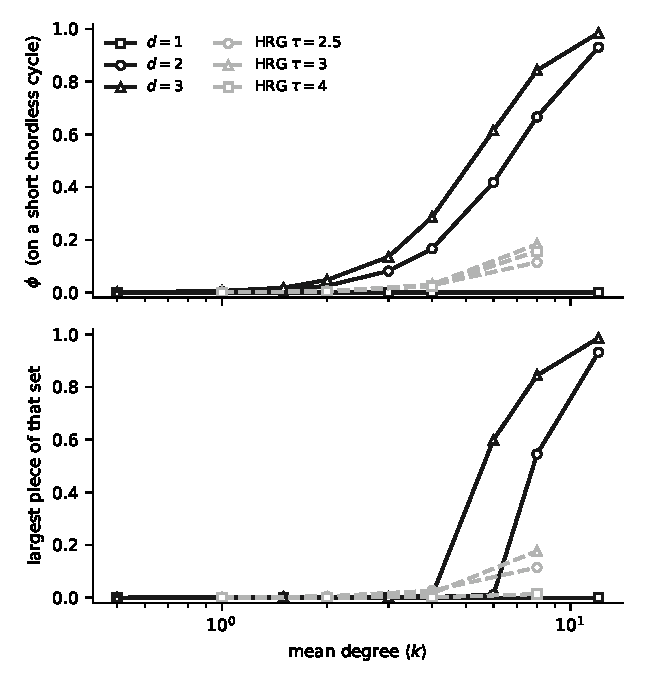
\includegraphics[width=\linewidth]{figs/fig-acyclicity.pdf}
\caption{\textbf{Where the clique family stops being locally acyclic.} Top:
$\phi$, the fraction of vertices on a chordless cycle of length four or five,
Eq.~\eqref{eq:phishort}, against mean degree at $n=20000$, for random
geometric graphs in $d=1$, $2$, $3$ (dark) and hyperbolic random graphs at
$\tau=2.5$, $3$, $4$ (light). Bottom: the largest connected piece of that
set, as a fraction of $n$. The line ($d=1$) is chordal and sits at zero
throughout; $d=2$ and $3$ are finite at every density and percolate well
above the graph's own threshold; the hyperbolic ensembles are small and
already one piece, the centre of the disc. Generated by
\code{figs/\allowbreak exactness.\allowbreak py} from
\code{statmech/\allowbreak probe/\allowbreak acyclicity.\allowbreak py}.}
\label{fig:acyclicity}
\end{figure}

\begin{figure}[t]
\centering
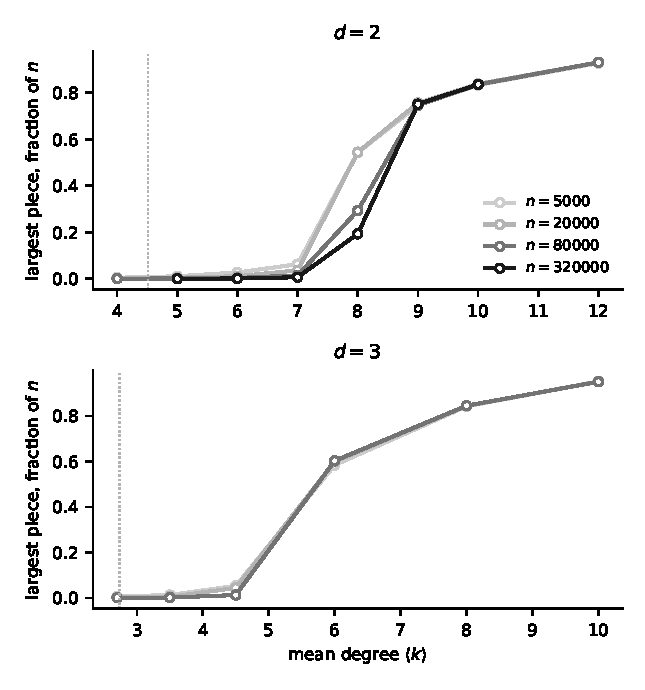
\includegraphics[width=\linewidth]{figs/fig-acyclicity-fss.pdf}
\caption{\textbf{Acyclicity percolation.} The largest island of vertices on
short chordless cycles, as a fraction of $n$, against mean degree at three
sizes, in $d=2$ (top) and $d=3$ (bottom). The dotted line is the mean degree
at which the graph itself acquires a giant component
\citep{penrose2003}. Between the two thresholds the islands are finite and
the meta-complex calculation is exact at a finite cost; above the second no
finite summation suffices. Generated by \code{figs/\allowbreak
exactness.\allowbreak py} from \code{statmech/\allowbreak probe/\allowbreak
acyclicity.\allowbreak py}, mode \code{fss}.}
\label{fig:fss}
\end{figure}

\begin{table}[t]
\centering\small
\begin{adjustbox}{max width=\linewidth}
\begin{tabular}{lrrrrrr}
\hline\hline
 & & & \multicolumn{2}{c}{$\phi$} & & \\
network & $\ave{k}$ & $C$ & real & rewired & piece & residue\\
\hline
Euroroad & 2.51 & 0.035 & 0.256 & 0.023 & 0.105 & 0.701\\
PDZ domains & 2.60 & 0.003 & 0.354 & 0.346 & 0.311 & 0.447\\
Power grid & 2.67 & 0.103 & 0.286 & 0.022 & 0.074 & 0.608\\
Yeast (Y2H) & 2.67 & 0.052 & 0.180 & 0.253 & 0.180 & 0.338\\
C. elegans 2007 & 2.71 & 0.017 & 0.227 & 0.306 & 0.227 & 0.309\\
C. elegans WI8 & 3.20 & 0.020 & 0.286 & 0.364 & 0.286 & 0.408\\
Human (Stelzl) & 3.85 & 0.006 & 0.388 & 0.457 & 0.385 & 0.500\\
Human (Vidal) & 4.32 & 0.035 & 0.492 & 0.526 & 0.492 & 0.586\\
Co-authorship & 4.82 & 0.431 & 0.077 & 0.773 & 0.047 & 0.129\\
Human (Figeys) & 5.79 & 0.008 & 0.517 & 0.526 & 0.517 & 0.531\\
Les Mis. scenes & 6.60 & 0.499 & 0.312 & 0.751 & 0.312 & 0.312\\
Football & 10.66 & 0.407 & 1.000 & 1.000 & 1.000 & 1.000\\
Facebook & 11.88 & 0.512 & 0.723 & 0.920 & 0.723 & 0.751\\
Collins yeast & 16.57 & 0.617 & 0.465 & 0.892 & 0.459 & 0.567\\
Jazz bands & 27.70 & 0.520 & 0.909 & 0.972 & 0.909 & 0.909\\
Hospital contacts & 30.37 & 0.588 & 1.000 & 1.000 & 1.000 & 1.000\\
\hline\hline
\end{tabular}

\end{adjustbox}
\caption{\textbf{Short chordless cycles on sixteen real networks.} The
largest component of each network; $C$ is the transitivity; $\phi$ is
Eq.~\eqref{eq:phishort} on the network and averaged over five
configuration-model rewirings of its degree sequence; ``piece'' is the
largest connected set of vertices on short chordless cycles, as a fraction
of $n$; ``residue'' is the GYO residue, which counts every cycle and is
uninformative. Group-generated networks sit far below their control,
interactomes on it, spatial networks far above it. Generated by
\code{figs/\allowbreak exactness.\allowbreak py} from
\code{statmech/\allowbreak probe/\allowbreak real\_\allowbreak
acyclicity.\allowbreak py}.}
\label{tab:realresidue}
\end{table}

\section{Conclusions}
\label{sec:exactness-conclusions}

The chygraph recursion is exact on an instance iff the clique family has a
join tree, which is iff the graph is chordal, which is iff leaf removal on the
incidence structure consumes everything. On an ensemble the condition is
local: no short chordless cycles, $\phi\to0$. Karrer--Newman satisfies it at
every branching ratio and one-dimensional geometry at every density.
Two-dimensional geometry never does, and is exact anyway at a finite cost up
to the acyclicity-percolation threshold, which sits well above the
percolation threshold of the graph. Hyperbolic random graphs fail only at
the centre, which is where their hubs and Sec.~\ref{sec:hrg}'s exponent are.
On real networks a rewired control sorts the short loops into those the
groups absorb, those the degree sequence makes and those the geometry makes,
and only the last are both real and finite.

What is not done is the ensemble calculation past the threshold: a message
indexed by separator type over a random join tree, the item
Sec.~\ref{sec:notdone} lists first. This chapter fixes what such a
calculation would have to average over --- the distribution of separators
and of islands --- and where it is needed at all.

\section{Checks}
\label{sec:exactness-checks}

\code{figs/\allowbreak exactness.\allowbreak py} runs, before it draws
anything: GYO reduction of the maximal cliques leaves no residue iff
\code{networkx} reports the graph chordal, on $200$ random graphs of twelve
vertices; the short-cycle finder of Eq.~\eqref{eq:phishort}, which works
from each vertex in time quadratic in its degree, marks the same vertices as
\code{networkx}'s chordless-cycle enumeration bounded at length five, on
$150$ random graphs; a one-dimensional geometric graph of $4000$ vertices at
$\ave{k}=30$ is chordal on the line and not on the ring; and on
sixteen-vertex geometric graphs at $\ave{k}=5$, region-graph message passing
over the maximal cliques returns $\ln Z$ to $10^{-6}$ on every
one-dimensional instance, all chordal, and is off by up to $1.4$ on the
two-dimensional ones, none chordal, at $\beta J=0.8$. The Karrer--Newman
count of Sec.~\ref{sec:whichexact} is the same script's
\code{check\_\allowbreak karrer\_\allowbreak newman}. The sweeps behind the
figures and the table are cached in \code{statmech/\allowbreak
probe/\allowbreak results/} and take about an hour and a half; the real
networks a few minutes.
